\documentclass[dvipdfmx]{jsarticle}
\usepackage[T1]{fontenc}
\usepackage[dvipdfmx]{hyperref}
\usepackage{lmodern}
\usepackage{latexsym}
\usepackage{amsfonts}
\usepackage{amssymb}
\usepackage{mathtools}
\usepackage{amsthm}
\usepackage{multirow}
\usepackage{graphicx}
\usepackage{wrapfig}
\usepackage{here}
\usepackage{float}
\usepackage{ascmac}
\usepackage{url}

\title{統計学1 中間課題 答案(再提出)}
\author{文理学部 情報科学科\\5419045 高林 秀}
\date{\today}

\begin{document}

\maketitle

\begin{abstract}
    本稿は、後期総合教育科目である統計学1の中間課題として与えられた、健康診断データの分析に関するレポートである。\par 
    平均や、標準偏差といった各種指標数値の計算にはPythonのライブラリであるPandasを用いて計算を行った。また、グラフの描画にはmatplotlibを使用した。\par 
    はじめに、各数値データ(年齢、身長、体重、最大血圧、最小血圧)に関して、それぞれ平均や標準偏差、度数分布表、ヒストグラムを作成し、元データ全体がどのような分布になっているかについて考察した。 
    その後、各数値(量的)データと質的データ(以降は「血圧判定」「心電図判定」を指す)の関連性を調べるため、相関比を算出し、結果から導かれることを考察した。
    その後、質的データ同士の関連性をクラメールの関連係数を用いて考察した。\par 
    最後に、算出した各種指標値の結果から、どの属性が質的データに影響を与えているのかを考察した。
\end{abstract}
\tableofcontents

\section{各データの概要}

    この章では、健康診断データの全体像を把握するため、平均や標準偏差、ヒストグラム、クロス集計表を用いて、各データの分布を可視化した。\par
    \subsection{各数値データの概要}
    まず、以下の表に性別を区別しない場合、男性のみのデータ、女性のみのデータでそれぞれの平均や標準偏差、最大値、最小値を算出した。
    \begin{table}[H]
        \caption{性別の区別がない場合の平均・標準偏差・最大,最小値}
        \centering
        \begin{tabular}{lccccc}
            & \multicolumn{1}{r}{年齢} & \multicolumn{1}{r}{身長(cm)} & \multicolumn{1}{r}{体重(kg)} & \multicolumn{1}{r}{最大血圧(mmHg)} & \multicolumn{1}{r}{最小血圧(mmHg)} \\
        平均   & 41.3                   & 162.5                  & 60.3                   & 124.9                    & 89.4                     \\
        標準偏差 & 12.1                   & 10.2                   & 9.4                    & 9.2                      & 15.2                     \\
        最大値  & 67.0                   & 185.0                  & 75.0                   & 144.0                    & 129.0                    \\
        最小値  & 23.0                   & 141.0                  & 43.0                   & 105.0                    & 65.0                     \\
        \hline
        総数 & 50 &  &  &  &  

    \end{tabular}
    \end{table}
    \begin{table}[H]
        \caption{男性のみのデータの平均・標準偏差・最大,最小値}
        \centering
        \begin{tabular}{lccccc}

            & \multicolumn{1}{r}{年齢} & \multicolumn{1}{r}{身長(cm)} & \multicolumn{1}{r}{体重(kg)} & \multicolumn{1}{r}{最大血圧(mmHg)} & \multicolumn{1}{r}{最小血圧(mmHg)} \\
        平均   & 40.0                   & 170.0                  & 66.0                   & 126.6                    & 87.0                     \\
        標準偏差 & 11.2                   & 6.2                    & 5.6                    & 9.3                      & 13.9                     \\
        最大値  & 67.0                   & 185.0                  & 75.0                   & 75.0                     & 125.0                    \\
        最小値  & 23.0                   & 159.0                  & 53.0                   & 115.0                    & 65.0                     \\
        \hline
        総数 & 24 &  &  &  & 
    \end{tabular}
    \end{table}
    \begin{table}[H]
        \caption{女性のみのデータの平均・標準偏差・最大,最小値}
        \centering
        \begin{tabular}{llllll}
            & \multicolumn{1}{r}{年齢} & \multicolumn{1}{r}{身長(cm)} & \multicolumn{1}{r}{体重(kg)} & \multicolumn{1}{r}{最大血圧(mmHg)} & \multicolumn{1}{r}{最小血圧(mmHg)} \\
        平均   & 41.7                   & 155.7                  & 55.0                   & 123.3                    & 91.6                     \\
        標準偏差 & 13.0                   & 8.2                    & 9.2                    & 8.9                      & 16.3                     \\
        最大値  & 65.0                   & 172.0                  & 75.0                   & 143.0                    & 129.0                    \\
        最小値  & 23.0                   & 141.0                  & 43.0                   & 105.0                    & 65.0                    \\
        \hline
        総数 & 26 &  &  &  &
        \end{tabular}
    \end{table}
    続いて、上記の3パターンで、各数値データのヒストグラムを示す。度数分布表は画像のサイズが大きい為、付録に記載する。
    \begin{figure}[H]
        \centering
        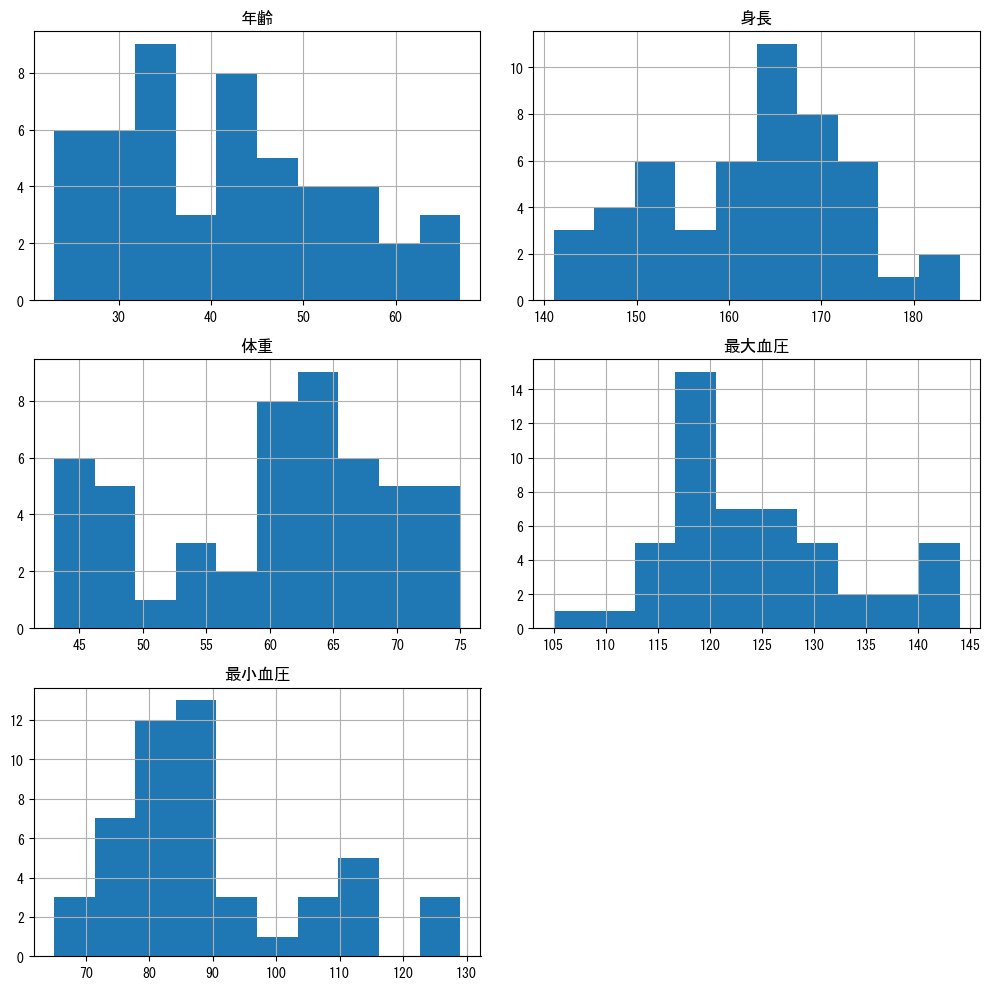
\includegraphics[scale=0.6]{./images/allgender/hist.png}
        \caption{全性別でのヒストグラム}
    \end{figure}
    \begin{figure}[H]
        \centering
        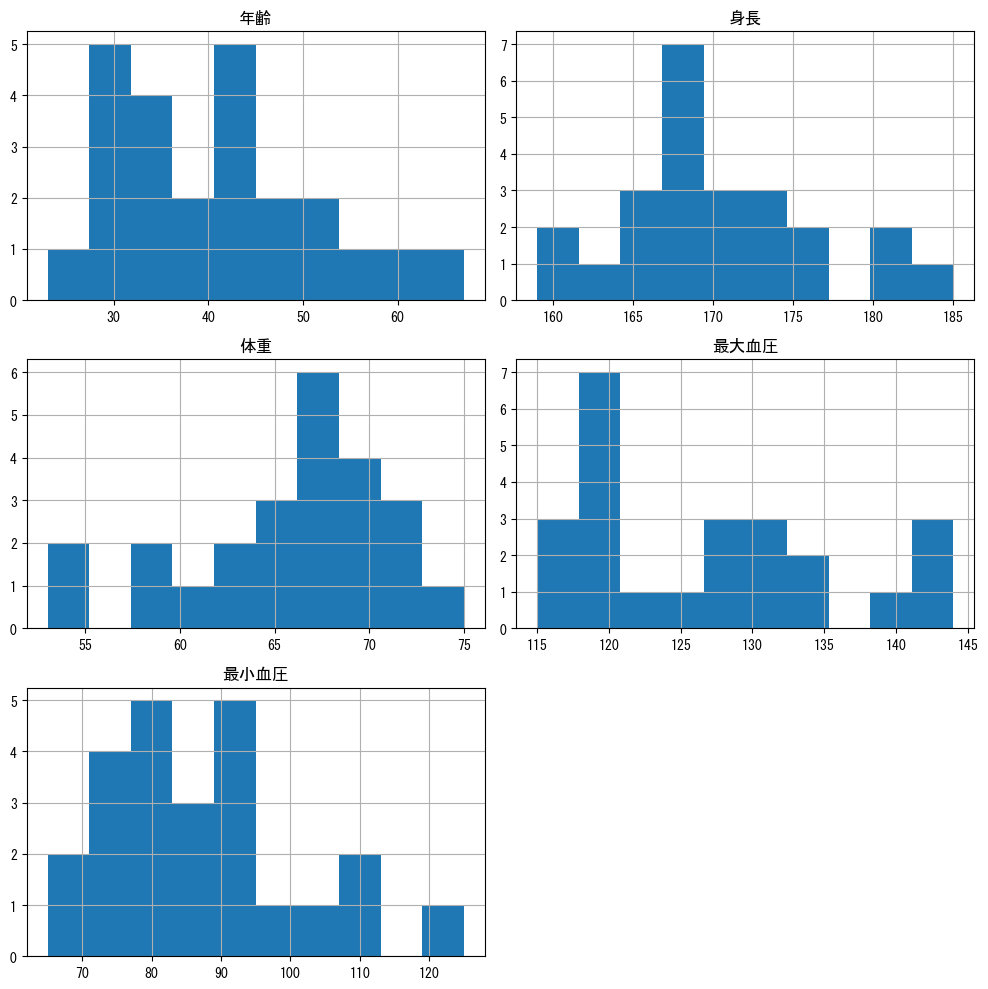
\includegraphics[scale=0.6]{./images/male/hist.png}
        \caption{男性データのヒストグラム}
    \end{figure}
    \begin{figure}[H]
        \centering
        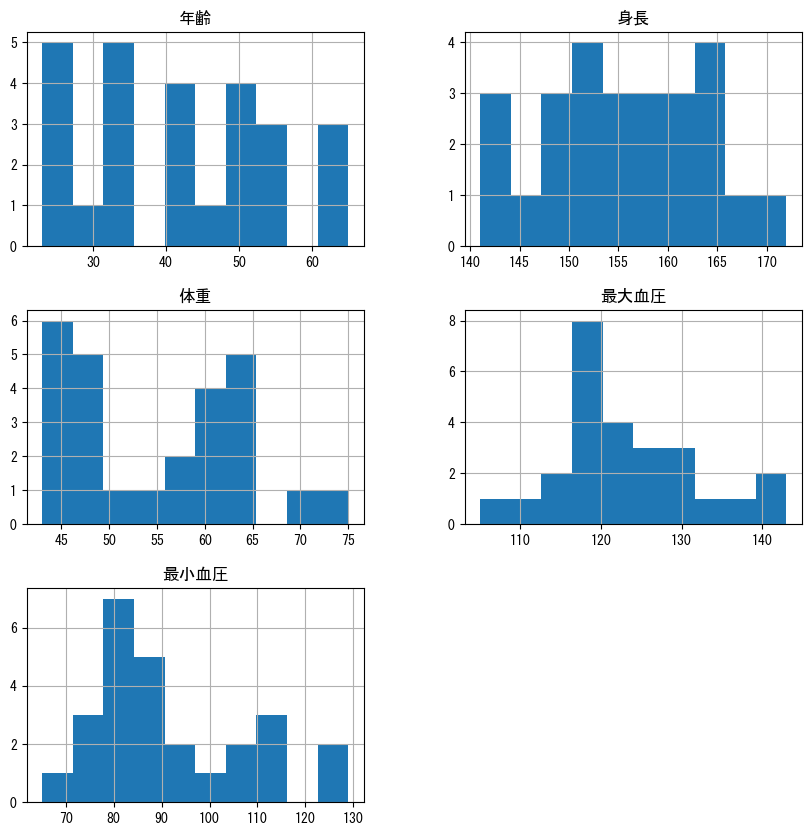
\includegraphics[scale=0.6]{./images/female/hist.png}
        \caption{女性データのヒストグラム}
    \end{figure}
    \subsubsection{年齢ごとの身長・体重・最大,最小血圧値の対応}
    続いて、年齢ごとの身長・体重・最大,最小血圧値の推移を折れ線グラフで可視化した。その結果を以下に示す。
    \begin{figure}[H]
        \centering
        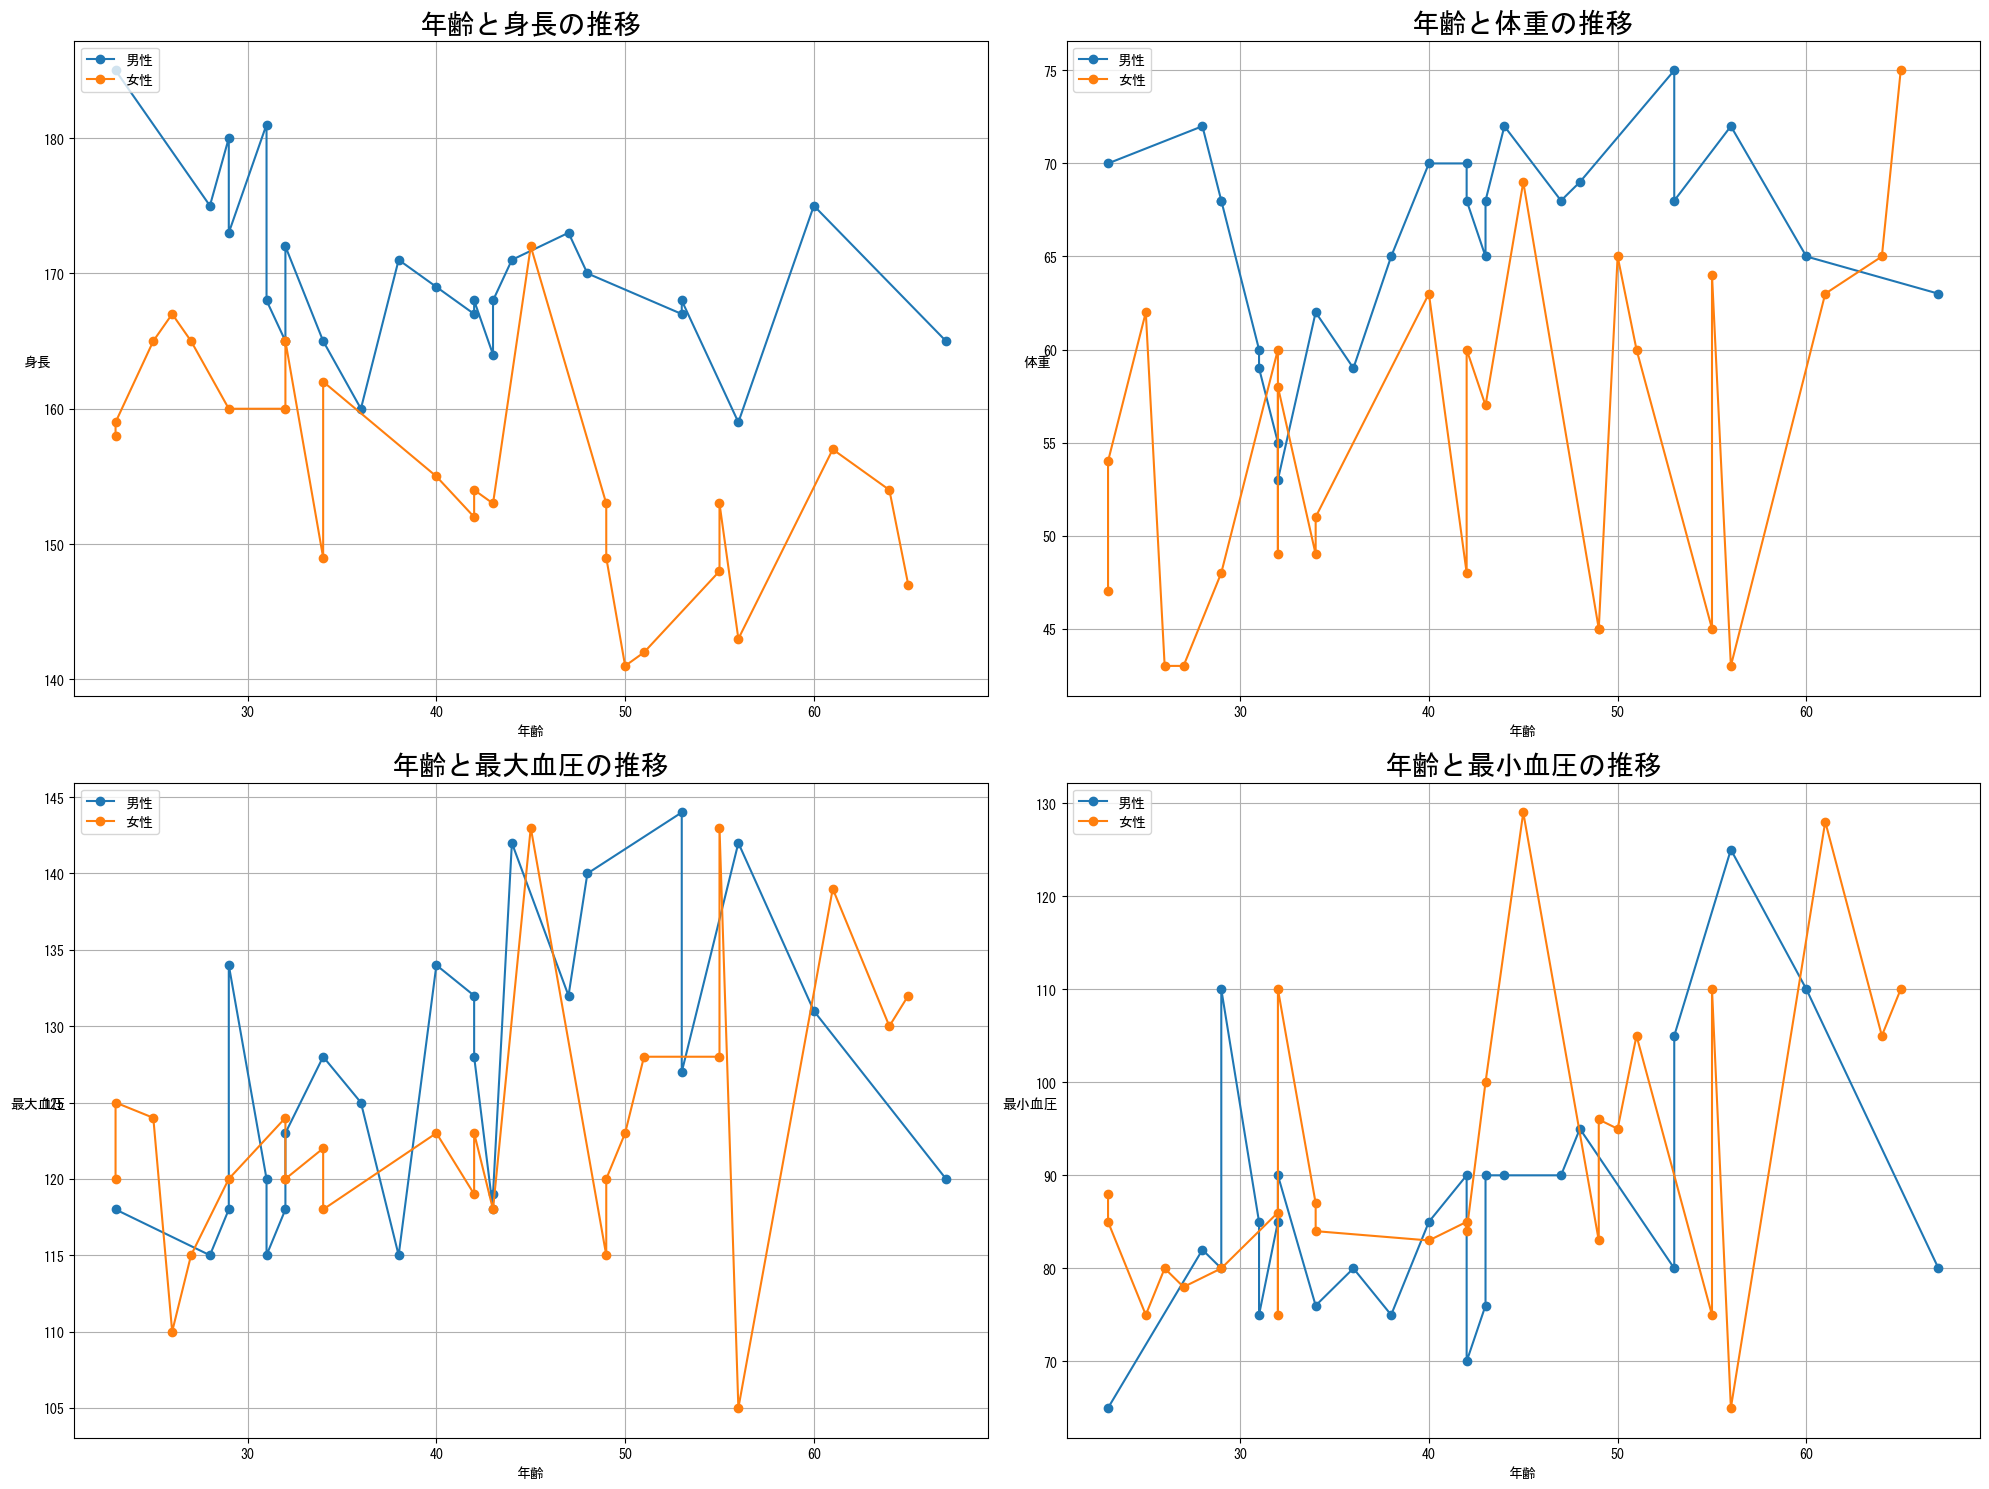
\includegraphics[scale=0.32]{images/allgender/age_tarnsition.png}
        \caption{年齢ごとの身長・体重・最大,最小血圧値の対応}
    \end{figure}
    このグラフから、本課題で使用したデータにおいて、年齢とそれ以外の各数値データの関係性に関して以下のことが言える。以下の考察はあくまで本データに対してのみであり、一般的なこととは限らない。
    \paragraph{年齢と身長}
    男性の場合は、年齢が上昇するにつれて全体として身長が下がっている傾向があるのが分かる。30代以下の人の身長の値は大体180cm~170cmの間であるのに対し、50代以上になると160cm~170cmの間の人が多く、年齢が大きくなるにつれて身長が下がっていく傾向がある。
    また、一般的に「高身長」といわれる身長175cm以上の人は、今回のデータでは30代以下がほとんどで、それ以上になると170cm程度の人が多いことが分かる。\par
    女性の場合も同様で、年齢が上昇するにつれて全体として身長が下がっている傾向があるのが分かる。30代以下の人の身長の値は大体160cm~170cmの間であるのに対し、50代以上になると140cm~150cmの間の人が多く、年齢が大きくなるにつれて身長が下がっていく傾向がある。\par
    また、性別によって、同じ年代でも身長大きさにはかなり開きがあることがこのグラフから明らかになった。特に、30代以下の人と、50代以上の人のデータにおいて、男性の身長は女性の身長よりも大きい傾向があることが分かる。
    \paragraph{年齢と体重}
    男性の場合は、女性に比べ比較的年代ごとに体重は同じような値をとっていることがグラフから分かる。例えば、40代~50代の人は大体体重65kg~70kgの間にある人が多い。反対に、女性の場合は同じ年代の人同士でも、体重の値に明かな開きがあることが分かる。
    例えば40代~50代の人は、体重の値が、下は45kg程度で上は70kg弱といったように、体重の値にかなりの開きがある。\par 
    また、男性の場合は、50代後半の人から、体重の値が下がっていく傾向にあるのに対し、女性の場合は反対に増えているのが分かる。この原因として以下の文章の現象が関係していそうなので引用する。
    \begin{quote}
        閉経を迎えると女性ホルモンよりも男性ホルモン優位となることが関係し、中性脂肪をため込みやすい体質に変化。また、基礎代謝量の減少により60代を超えるとBMIは23台へと数値が上がる。
    \end{quote}
    ※引用元:\url{https://womanslabo.com/c-marketing-tips-190614-8} \par 
    一般的に個人差はあるが、女性の閉経時期は50代中ごろと言われている。引用文にある通り、閉経によるホルモンバランスの変化により中性脂肪を貯えやすい体質に変化し、加齢による基礎代謝量の減少により体重が上昇していると考えられる。実際にグラフから、50代後半の人の体重データは、それ以下の年代の人に比べて上昇傾向にあるのが分かる。
    \paragraph{年齢と最大,最小血圧}
    最大,最小血圧の値に関しては、身長、体重のグラフと異なり、若干重なっているように見え、あまり開きがない。これは、男性と女性の最大,最小血圧の値にはあまり乖離がないことを意味する。
    しかし、体重の部分でも述べたように、一般的に女性の閉経が始まるとされる50代後半以降のグラフをみると、極端に男性と女性の血圧値に開きがある。加えて、その年代以降の女性は、それ以前の年代の人よりも血圧値が高めになっているのが分かる。
    その原因として、以下の文章の現象が関係していそうなので引用する。
    \begin{quote}
        閉経によりエストロゲンに変換されなくなり、相対的に男性ホルモンが多くなります。すると自律神経の1つである交感神経の働きが活発化したり、血圧上昇を促すレニンというホルモンの産生が上昇したりします。つまり閉経にともなう相対的男性ホルモンの働きの増加も高血圧を引き起こす原因になります。
    \end{quote}
    ※引用元:\url{https://www.senshiniryo.net/column_a/29/index.html#:~:text=%E9%96%89%E7%B5%8C%E3%81%AB%E3%82%88%E3%82%8A%E3%82%A8%E3%82%B9%E3%83%88%E3%83%AD%E3%82%B2%E3%83%B3%E3%81%AB%E5%A4%89%E6%8F%9B,%E5%BC%95%E3%81%8D%E8%B5%B7%E3%81%93%E3%81%99%E5%8E%9F%E5%9B%A0%E3%81%AB%E3%81%AA%E3%82%8A%E3%81%BE%E3%81%99%E3%80%82} \par
    以上の文にあるように、一般的に女性の場合、閉経にともなう相対的男性ホルモンの働きの増加により血圧が上昇傾向にあるようだ。このことから、グラフの「50代後半以降のグラフをみると、極端に男性と女性の血圧値に開きがある。加えて、その年代以降の女性は、それ以前の年代の人よりも血圧値が高めになっている」部分に関して納得が出来る。
    \subsection{質的データ(血圧判定、心電図判定)の概要}
\section{各数値データの相関比}
\section{各属性のクラメールの関連係数}
\section*{付録}
    \subsection*{計算機環境}
    \subsection*{図表一覧}
    \subsection*{ソースコード}
\end{document}